%!TEX root = main_arduino_intro.tex

\chapter{Arduino Micro Pinout}\label{app:pinout}

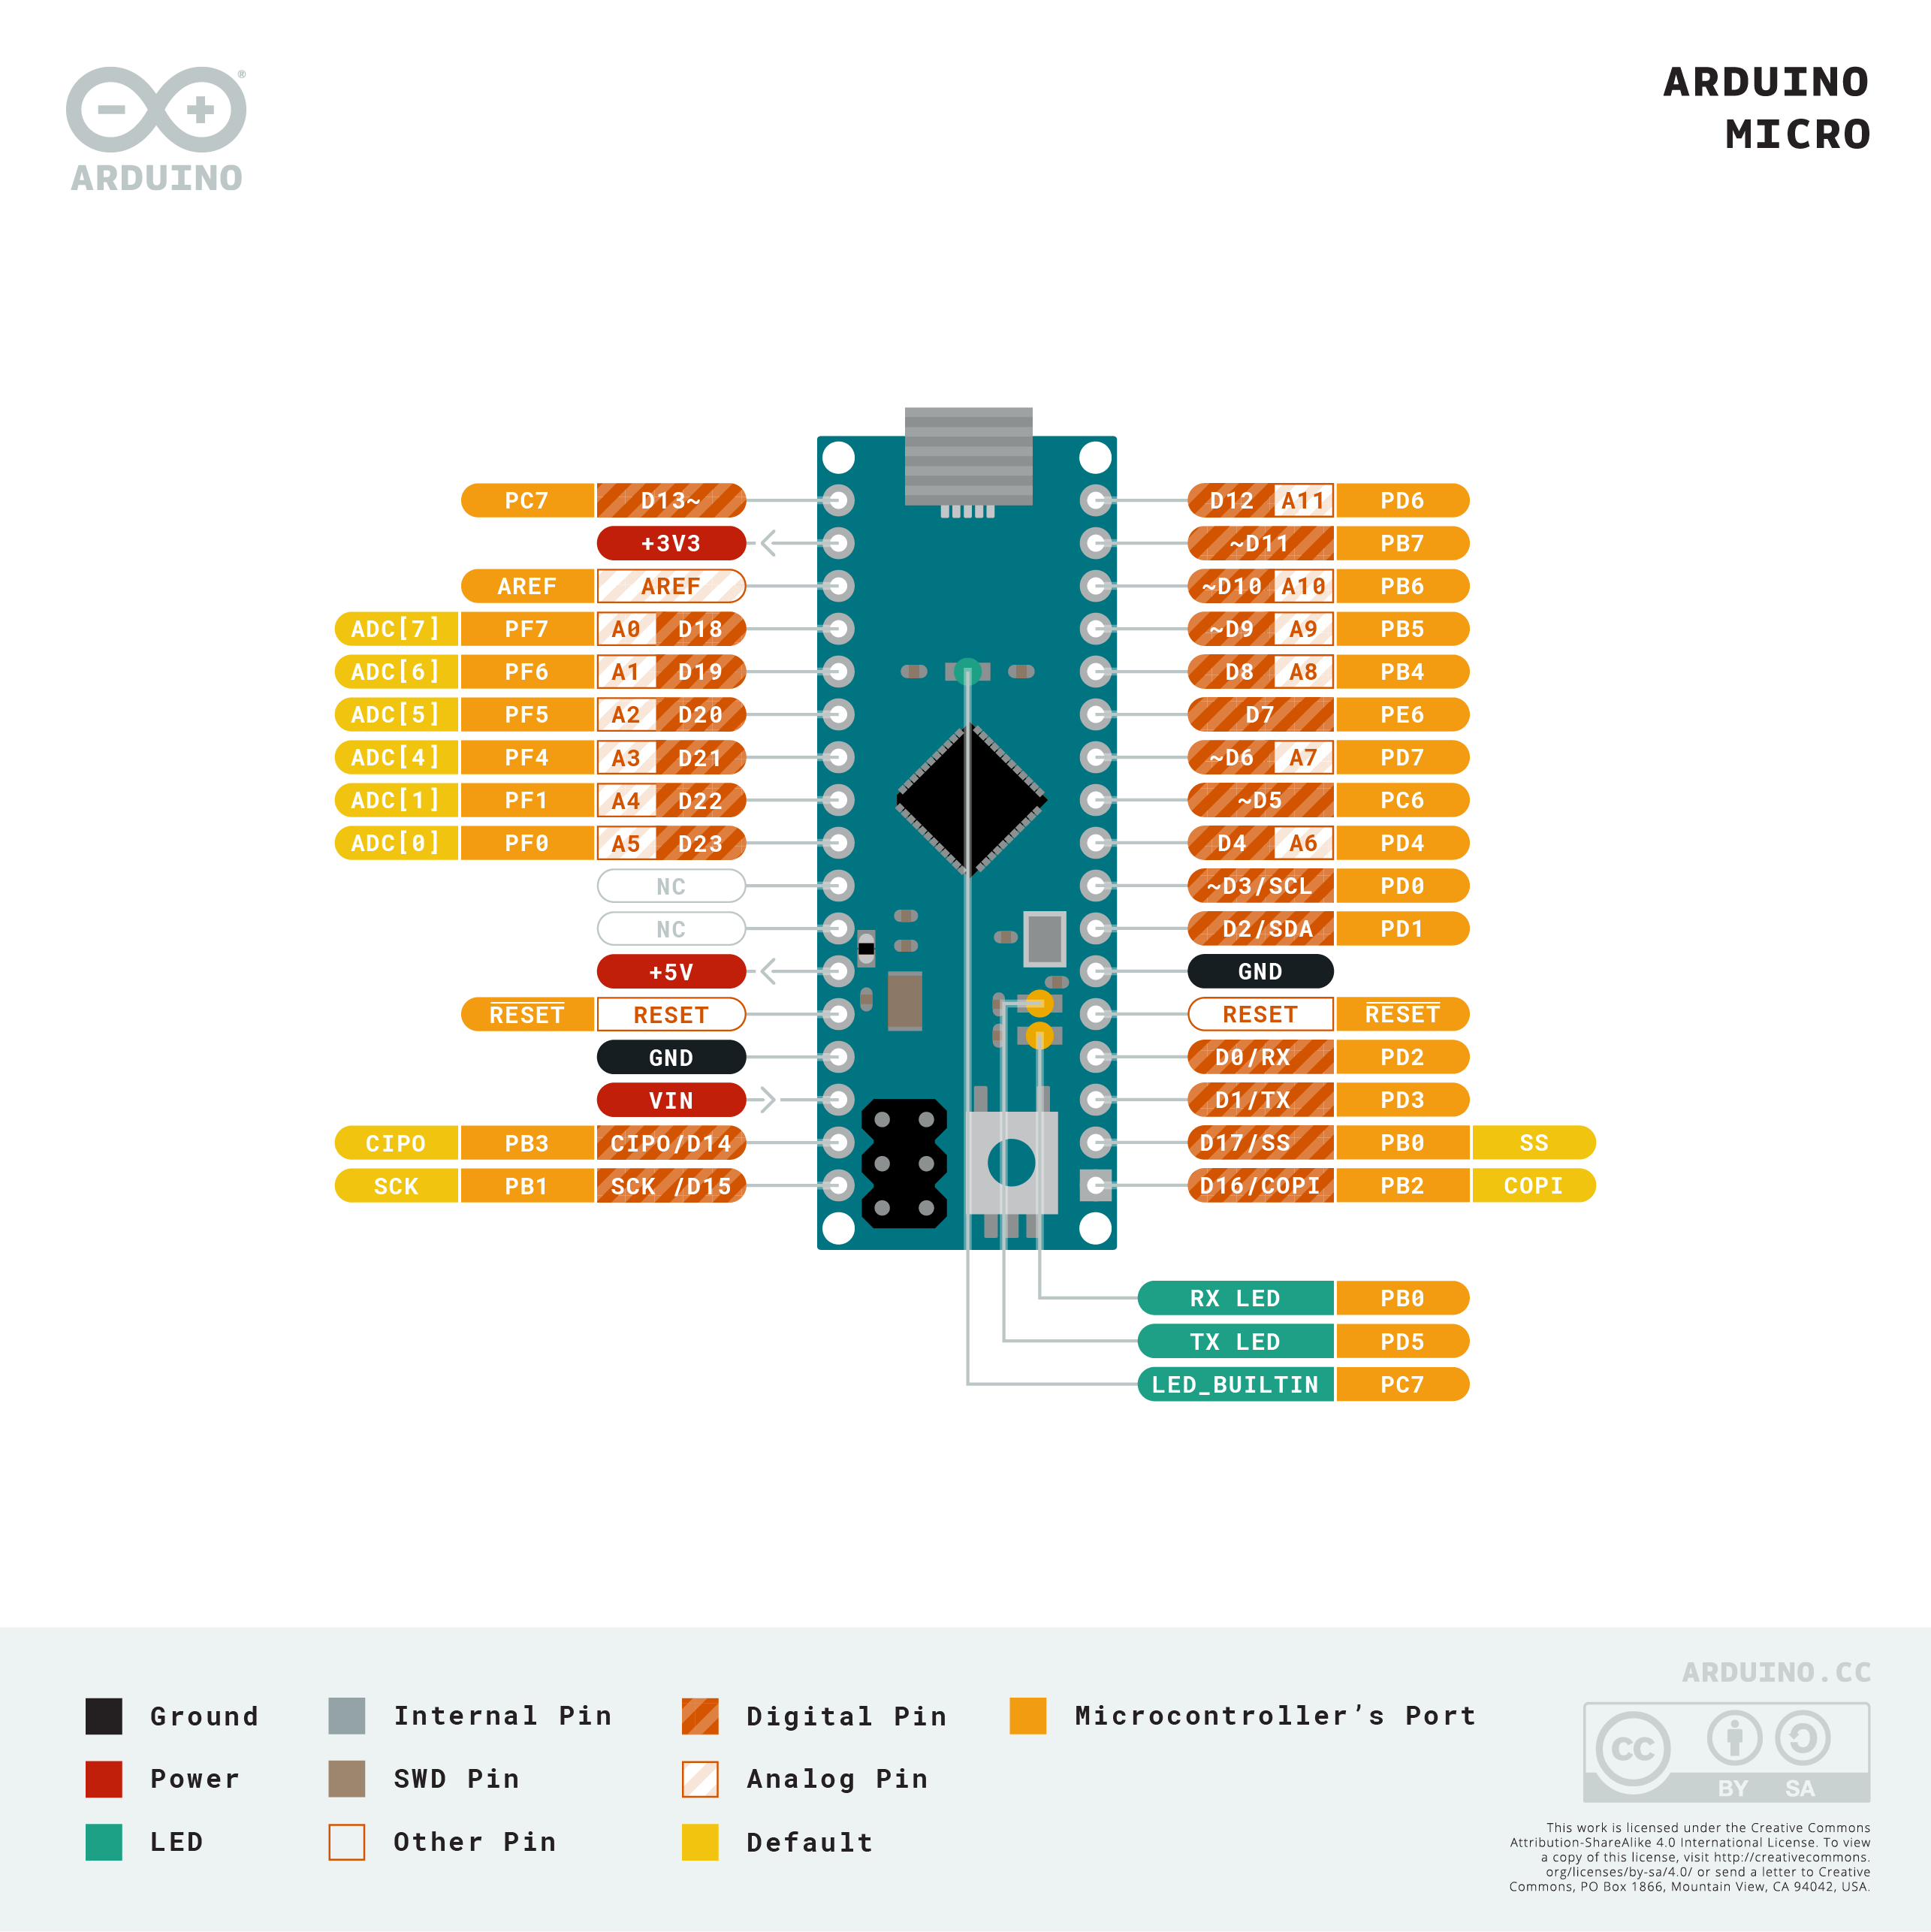
\includegraphics[width=\textwidth]{graphics/appendix/arduino_pinout.png}

%%%%%%%%%%%%%%%%%%%%%%%

\chapter{\Acf{bom}}

The following table states all components used in this workshop. It assumed that soldering stations and supplies are provided.

\begin{center}
\begin{tabular}{lllcr}
\hline
\textbf{Component}  &   \textbf{Supplier}   &   \textbf{Article \#} &   \textbf{Amount} &   \textbf{Cost total} \\
\hline\hline
Arduino Micro       &   \href{https://www.digikey.com/en/products/detail/arduino/A000053/4486332}{Digikey}             &   A000053             &   1   &   \$20.70 \\
USB Cable           &   \href{https://www.digikey.com/en/products/detail/cui-devices/CBL-UA-MUB-1/9838595?s=N4IgTCBcDaIIwAYwFoCsBOALAZmQOQBEQBdAXyA}{Digikey}             &   102-5943-ND         &   1   &   \$2.55 \\
Breadboard          &   \href{https://www.adafruit.com/product/239}{Adafruit}   &   239     &   1   &   \$5.95  \\
Breadboard wires    &   \href{https://www.adafruit.com/product/153}{Adafruit}   &   153     &   1   &   \$4.95  \\
\ac{led} red        &   \href{https://www.digikey.com/en/products/detail/broadcom-limited/HLMP-3600/637603?s=N4IgTCBcDaIKwEYBsBaBBmdBOFA5AIiALoC%2BQA}{Digikey}    &   516-1339-ND         &   1   &   \$0.81  \\
\ac{led} green      &   \href{https://www.digikey.com/en/products/detail/broadcom-limited/HLMP-3962/637598?s=N4IgTCBcDaIKwEYBsBaBBmdAWFA5AIiALoC%2BQA}{Digikey}     &   516-1334-ND &   1   &   \$0.78 \\
Buttons             &   \href{https://www.adafruit.com/product/367}{Adafruit}   &   367     &   1   &   \$2.50  \\
Resistors 1\,k$\Omega$ & \href{https://www.adafruit.com/product/4294}{Adafruit}  &   4294    &   1   &   \$0.75  \\
Resistors 10\,k$\Omega$ & \href{https://www.adafruit.com/product/2784}{Adafruit}  &   2784    &   1   &   \$0.75  \\
Display             &   \href{https://www.adafruit.com/product/1002}{Adafruit}   &   1002    &   1   &   \$10.95    \\
Thermistor          &   \href{https://www.adafruit.com/product/372}{Adafruit}   &   372     &   1   &   \$4.00  \\
\Ac{tec}            &   \href{https://www.adafruit.com/product/1335}{Adafruit}   &   1335    &   1   &   \$34.95     \\
MOSFET              &   \href{https://www.adafruit.com/product/355}{Adafruit}   &   355     &   1   &   \$1.75  \\
12\,V power supply  &   \href{https://www.adafruit.com/product/352}{Adafruit}   &   352     &   1   &   \$24.95     \\
Power jack adapter  &   \href{https://www.adafruit.com/product/368}{Adafruit}   &   368     &   1   &   \$2.00  \\
\hline
\textbf{Total cost:}    &   &   &   &   \textbf{\$118.34}   \\
\hline
\end{tabular}
\end{center}

%%%%%%%%%%%%%%%%%%%%%%%

\chapter{Open source design tools}

\section{Calculators}
\begin{itemize}
    \item \textbf{Heat sink calculator} to determine if you need a heat sink or not. \url{https://daycounter.com/Calculators/Heat-Sink-Temperature-Calculator.phtml} 
\end{itemize}

\section{Designing}
\begin{itemize}
    \item \textbf{EasyEDA}{Online designer for \acp{pcb} with large library of components and direct ordering possibilities. \url{https://easyeda.com/}}
    \item \textbf{Fritzing} Makes electronics design accessible. Easy and simple interface to draw some of your own setups, quick to get started with. Suppliers such as Adafruit have Fritzing libraries with components that you can import. \url{https://fritzing.org/}
    \item \textbf{KiCad} Cross-platform electronics design suite. \url{https://www.kicad.org/}
\end{itemize}

\section{Virtual Hardware}
\begin{itemize}
    \item \textbf{TinkerCAD} Electronic playground from Autodesk. Allows you to virtually set up electronic components and write / test code for them. \url{https://www.tinkercad.com/}
\end{itemize}

%%%%%%%%%%%%%%%%%%%%%%%

\chapter{Full wiring diagram}

\begin{figure}[h!]
    \centering
    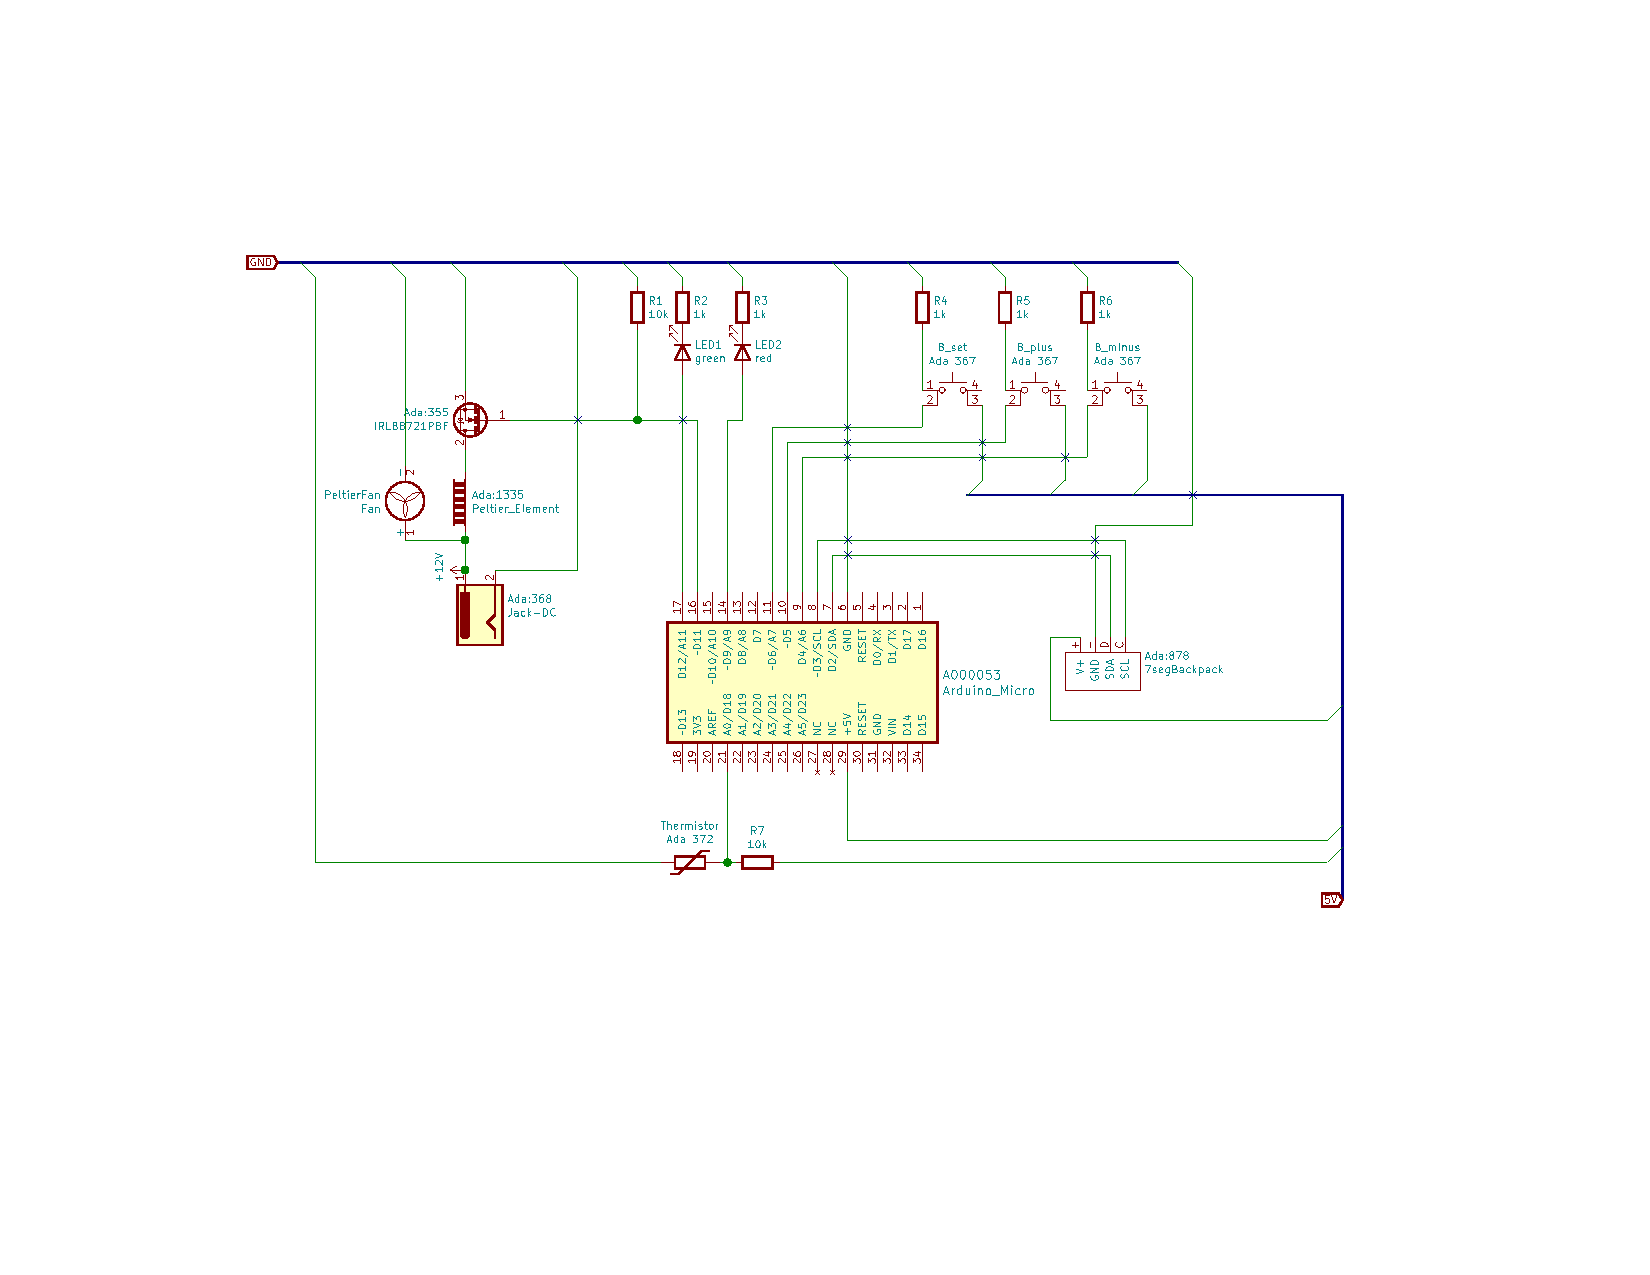
\includegraphics[width=\textwidth]{graphics/appendix/diagram_full_assembly.pdf}
    \caption{Full wiring diagram of the final project. All \href{https://www.kicad.org/}{KiCAD} files can be found on \href{https://github.com/galactic-forensics/workshop_arduino_electronics/tree/main/kicad}{GitHub}.}
    \label{fig:appendix:full_wiring_diagram}
\end{figure}
